
\section{Postřiky}
Zvolili jsme kompletní řešení postřiků od fitmy BASF\footnote{BASF je německá agrochemická firma, která patří k 
největším na světě.\\https://www.agro.basf.cz/agroportal/cz/cs/startpage.html.}.
Pro určení přibližné ceny jednotlivých postřikových přípravků použijeme ceny existujícího eshopu obchod.agrokop.cz\footnote{AGROKOP CZ, a.s. Třebíč}.
\begin{figure}[ht!]
\centering
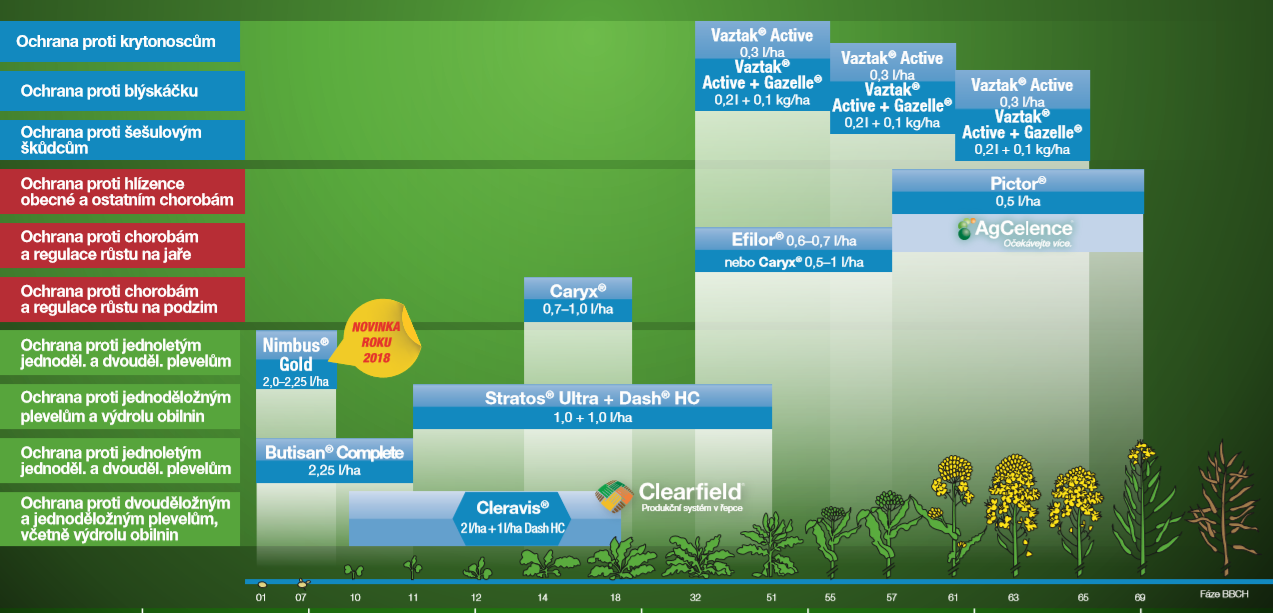
\includegraphics[width=170mm]{img/postriky}
\caption{Ochrana řepky proti škodlivým činitelům firmy BASF \label{basf_postriky}}
\end{figure}
Používané přípravky se dělí do několika skupin, to je důležité hlavně kvůli informaci o mísitelnosti jednotlivých přípravků.
\begin{itemize}
  \item Listová hnojiva.
  \item Fungicidy.
  \item Insekticidy.
  \item Herbicidy.
  \item Graminicidy.
\end{itemize}

\subsection{Ochrana proti krytonoscům, blýskáčku a šešulovým škůdcům}
Použitý přípravek se nazývá Vaztak Active\footnote{Vaztak je přípravek německého výrobce BASF: \\\url{\detokenize{
https://www.agro.basf.cz/agroportal/cz/cs/crop_protection/vyhled_v_n__p__pravk__podle_parametr_/product_details_24923.html
}}
\\\url{\detokenize{
https://www.agro.basf.cz/agroportal/cz/media/migrated/product_files/charakteristiky/CH_Vaztak_Active.pdf}}.}.
Vaztak Active je vysoce účinný světlostabilní pyrethroidní insekticid, určený proti 
některým  druhům  žravého  a  savého  hmyzu,  jeho  larvám  a  vajíčkům.  Účinkuje  
jako dotykový a požerový jed. Není systémovým přípravkem a je proto třeba do statečného množství vody k zabezpečení dobrého krycího postřiku. Přípravek je 
stabilní vůči světlu a má nízkou rozpustnost ve vodě, proto má dobrý reziduální 
účinek na povrchu listů. Povlak Vaztaku Active je odolný vůči dešti za předpokladu, že postřik zaschne dříve, než začne pršet.

\begin{itemize}
  \item Spotřeba 0,3l/ha. * 3 za každé období postřiku.
  \item Doporučené množství vody 200–600 l/ha (polní plodiny, zelenina), 200–1000 l/ha (prostorové plodiny) 
  \item Kategorie Insekticidy.
  \item Mísit lze se vším.
  \item Cena 815 bez DPH za litr.
\end{itemize}

\subsubsection{Aplikace postřiku}

Lze konstatovat, že aplikace proti krytonosci řepkovému je v vhodná po 9 až 11 dní po prvním vrcholu náletu do porostu, u krytonosce čtyřzubého obvykle o 7 až 14 dní později. Předčasné aplikace jsou neúčinné, protože likvidujeme pouze nálety samců a samice nepostihujeme. Proto je vhodné pred postřikem se presvedčit, zda je hektár dostatečne infikován než použijeme postřik.

\subsection{Ochrana proti hlízence obecné a ostatním chorobám}
Použitý přípravek se nazývá Pictor\footnote{Pictor je přípravek německého výrobce BASF: \\\url{\detokenize{
https://www.agro.basf.cz/agroportal/cz/cs/crop_protection/vyhled_v_n__p__pravk__podle_parametr_/product_details_1396.html
}}
\\\url{\detokenize{https://www.agro.basf.cz/agroportal/cz/media/migrated/information_material/brochures_products_1/brochures_products/2014/Pictor_Errata.pdf}}
.}.
Vysokou preventivní a kurativní účinnost zajištuje vyvážený poměr dvou kompatibilních látek - boscalidu a dimoxystrobinu, které působí na dýchací procesy houbových organizmů.
\begin{itemize}
  \item Spotřeba 0,5l/ha.
  \item Doporučené množství vody 200-400l/ha.
  \item Kategorie Fungicidy.
  \item Mísit lze se vším.
  \item Cena 3280 bez DPH za litr.
  \item Hlízenka obecná může způsobit výnosové 
ztráty až 30 \%
\end{itemize}

\subsubsection{Aplikace postřiku}
Postřik je ochranný, preventivní. Aplikuje se jednou. Pro úspěšné použití fungicidů proti hlí-
zence obecné bylo vždy nutné směřovat aplikaci do doby plného květu. 
Oproti stávajícím fungicidům se Pictor vyznačuje vyšší flexibilitou použití. Díky dlouhodobému působení účinných látek je
možné použít Pictor již v době krátce před květem až do konce kvetení.


\subsection{Ochrana proti chorobám a regulace růstu na jaře}
Použitý přípravek se nazývá Efilor\footnote{Efilor je přípravek německého výrobce BASF: \\\url{\detokenize{
https://www.agro.basf.cz/agroportal/cz/cs/crop_protection/vyhled_v_n__p__pravk__podle_parametr_/product_details_72192.html
}}.}.
Efilor zajišťuje vynikající ochranu proti houbovým chorobám a kompaktní porosty s ideální architekturou, které díky tomu rovnoměrně kvetou a dozrávají.
\begin{itemize}
  \item Spotřeba 0,6l/ha.
  \item Doporučené množství vody 150-400l/ha.
  \item Kategorie Fungicidy.
  \item Mísit nelze pouze pýrohubné dávky u Graminicidů.
  \item Cena 1399 bez DPH za litr.
\end{itemize}

\subsubsection{Aplikace postřiku}
Preventivně nebo co nejdříve na počátku výskytu choroby.

\subsection{Ochrana proti chorobám a regulace růstu na podzim}
Použitý přípravek se nazývá Caryx\footnote{Caryx je přípravek německého výrobce BASF: \\\url{\detokenize{
https://www.agro.basf.cz/agroportal/cz/cs/crop_protection/vyhled_v_n__p__pravk__podle_parametr_/product_details_1446.html
}}
\\\url{\detokenize{
https://www.agro.basf.cz/agroportal/cz/media/migrated/information_material/brochures_products_1/brochures_products/2014/Caryx_Errata.pdf
}}.}.
Pouze  homogenní  porost  řepky na jaře na začátku prodlužovacího růstu rostlin umožňuje vytvoření  ideální  architektury  porostu 
později v sezóně a tím rovnoměrného kvetení a tvorby šešulí. 
Rovnoměrný  vývoj,  trvalé  zkrácení  a  zesílení  stonků  a  z  toho 
vyplývající odolnost k poléhání – to jsou vynikající výsledky, které přináší použití přípravku Caryx. 
Výsledkem je vyšší hmotnost tisíce semen. Stejnoměrné dozrávání zvyšuje i kvalitu výnosu a snižuje vlhkost sklízených semen.
\begin{itemize}
  \item Spotřeba 0,75-1l/ha.
  \item Doporučené množství vody 150-400l/ha.
  \item Kategorie Fungicidy.
  \item Mísit nelze pouze pýrohubné dávky u Graminicidů.
  \item Cena 1009 bez DPH za litr.
\end{itemize}

\subsection{Ochrana proti jednoletým jednoděl. a dvouděl. plevelům}
První možný přípravek se nazývá Butisan Complete\footnote{Butisan Complete je přípravek německého výrobce BASF: \\\url{\detokenize{
https://www.agro.basf.cz/agroportal/cz/cs/crop_protection/vyhled_v_n__p__pravk__podle_parametr_/product_details_85632.html
}}.}.
\begin{itemize}
  \item Spotřeba 2-2,25l/ha.
  \item Doporučené množství vody 100-400l/ha.
  \item Kategorie Herbicidy.
  \item Mísit lze se vším.
  \item Cena 1016 bez DPH za litr.
\end{itemize}

\subsection{Ochrana proti jednoděložným plevelům a výdrolu obilnin}
Použitý přípravek se nazývá Stratos Ultra\footnote{Stratos Ultra je přípravek německého výrobce BASF: \\\url{\detokenize{
https://www.agro.basf.cz/agroportal/cz/cs/crop_protection/vyhled_v_n__p__pravk__podle_parametr_/product_details_1429.html
}}
\\\url{\detokenize{
https://www.agro.basf.cz/agroportal/cz/media/migrated/product_files/charakteristiky/CH_Stratos_Ultra.pdf
}}.}.
Stratos  Ultra  je  selektivní  systémový  herbicid,  jehož  účinná  látka  je  přijímána  
zelenými nadzemními částmi rostlin. Účinnost je proto zaručena i v suchých letech,  kdy  mohou  půdní  herbicidy  selhávat.  V  době  ošetření  mají  být  plevelné  
rostliny v plném růstu a vyvinuty tak, aby měly dostatek zelené hmoty pro přijetí 
potřebného množství účinné látky. Účinnost se projeví již za 3–4 dny po ošetření.
\begin{itemize}
  \item Spotřeba 1l/ha.
  \item Doporučené množství vody 200-300l/ha.
  \item Kategorie Herbicidy.
  \item Mísit nelze s listovým hnojivem Solubor.
\end{itemize}
Pomocný přípravek se nazývá Dash HC\footnote{Dash HC je přípravek německého výrobce BASF: \\\url{\detokenize{
https://www.agro.basf.cz/agroportal/cz/cs/crop_protection/vyhled_v_n__p__pravk__podle_parametr_/product_details_1441.html
}}.}.
\begin{itemize}
  \item Spotřeba 1l/ha.
  \item Doporučené množství vody 300l/ha.
\end{itemize}
Cena za 10l přípravku Stratos Ultra a 10l přípravku Dash HC je 6990 bez DPH.

\subsubsection{Aplikace postřiku}
Stratos Ultra se používá v ošetřovaných plodinách po vzejití lipnicovitých plevelů. Termín ošetření se řídí především růstovou fází plevelů, méně už růstovou fází 
kulturní plodiny. Teplé a vlhké počasí nebo příznivé růstové podmínky účinnost 
urychlují, sucho a nízké teploty ji naopak zpomalují. V oblastech s vysokou světelnou intenzitou je vhodnější ošetřovat v podvečerní době.


\subsection{Ochrana proti dvouděložným a jednoděložnám plevelům, včetně výdrolu obilnin}
Použitý přípravek se nazývá Cleravis\footnote{Cleravis je přípravek německého výrobce BASF: \\\url{\detokenize{
https://www.agro.basf.cz/agroportal/cz/cs/crop_protection/vyhled_v_n__p__pravk__podle_parametr_/product_details_55941.html
}}
\\\url{\detokenize{
https://www.agro.basf.cz/agroportal/cz/media/migrated/product_files/charakteristiky/CH_Cleravis.pdf
}}.}.
Selektivní postřikový herbicid ve formě tekutého suspenzního koncentrátu (SC)
k hubení jednoletých dvouděložných a jednoděložných plevelů včetně výdrolu 
obilnin v porostech řepky
\begin{itemize}
  \item Spotřeba 2l/ha.
  \item Doporučené množství vody 300-400l.
  \item Kategorie Herbicidy.
  \item Mísit nelze s Graminicidy.
\end{itemize}
Pomocný přípravek se nazývá Dash HC.
\begin{itemize}
  \item Spotřeba 1l/ha.
  \item Doporučené množství vody 300l/ha.
\end{itemize}
Cena za 10l přípravku Cleravis a 5l přípravku Dash HC je 11699 bez DPH.

\subsubsection{Aplikace postřiku}
Správný termín aplikace Cleravisu je obecně 
dán stádiem plevelů, ve kterém jsou citlivé k herbicidům, méně již růstovou fází 
řepky.
Maximální počet aplikací je 1x v plodině za vegetaci.
